\documentclass[10pt,twocolumn,letterpaper]{article}

\usepackage{wacv}
\usepackage{times}
\usepackage{epsfig}
\usepackage{graphicx}
\usepackage{amsmath}
\usepackage{amssymb}
\usepackage{booktabs}
\usepackage{xcolor}
\usepackage{listings}
\usepackage[pagebackref,breaklinks,colorlinks]{hyperref}
\usepackage[capitalize]{cleveref}

\lstset{basicstyle=\ttfamily\small, breaklines=true, columns=fullflexible,
  frame=none, backgroundcolor=\color{black!4},
  xleftmargin=4pt, xrightmargin=4pt, breakindent=0pt,
  postbreak=\mbox{{$\hookrightarrow$}\space}}

\def\wacvPaperID{*****}
\def\confName{WACV}
\def\confYear{2027}

\begin{document}
\raggedbottom

\title{Evidence-First VLM Cascades for Embedded Work-Zone State Estimation:\\
Hyper-Parameter Portability and the Cost of Specialization\\
\vspace{4pt}\large Supplementary Material}

\author{Anonymous WACV submission\\
Paper ID \wacvPaperID}
\maketitle

\appendix

\section{Reproducibility}
\label{supp:repro}

This supplement contains everything needed to reproduce the system short of the fine-tuned weights: the byte-exact prompts and parsing rules (\cref{supp:prompts}), the full corroboration lexicon and qualifier filter (\cref{supp:lexicon}), the Bayesian-filter emission/transition matrices and all hysteresis constants (\cref{supp:bayes}), the deployment configuration and quantization recipe (\cref{supp:deploy}), and the exact latency-honest evaluation protocol (\cref{supp:deploy}).  We release, as anonymized supplementary code, the camera-simulation harness, the paper-exact metric implementations, the ablation and debounce-sweep scripts, the ported detector+CLIP baseline, the video-level split files, and---new to this version---the evidence-dump and offline-replay calibration harness (\cref{supp:calib}), and the out-of-domain benchmark protocol and annotations (\cref{supp:ood})---enough to reproduce every table from cached predictions or from the engines.  The fine-tuned checkpoint and full training corpus will be released on publication.

\section{Exact prompt texts and parsing rules}
\label{supp:prompts}

All four channels share one model and one engine; a ``channel'' is exactly a (prompt, token-budget) pair.  The prompts below are byte-exact as sent to the model in every reported experiment.

\paragraph{\textsc{gate} (3 tokens; 2 in state-only mode).}
\begin{lstlisting}
Are there any road work indicators in this scene (cones, barriers, temporary signs, workers, work vehicles)? Answer Yes or No.
\end{lstlisting}
Parsing: a reply starting with \texttt{yes} $\to$ true; starting with \texttt{no}/\texttt{none} $\to$ false.  The fine-tuned model sometimes answers in its SFT counting template (``\texttt{2 temporary sign(s) detected \dots}''); a leading count $N$ parses as $N{>}0$.  Anything else parses as \emph{unknown} and is treated as gate-inactive for that cycle.

\paragraph{\textsc{sign} (15 tokens).}
\begin{lstlisting}
Read any temporary traffic control signs visible in this scene. What do they say?
\end{lstlisting}
No parsing beyond keyword matching (\cref{supp:lexicon}): the transcription itself is the evidence.  The binary alternative used in the ablation (\cref{supp:binary}) replaces this text entirely.

\paragraph{\textsc{ego} (8 tokens; 3 in state-only mode).}
\begin{lstlisting}
Regarding the road work zone, is the ego vehicle OUTSIDE, APPROACHING, or INSIDE the work zone? Answer with one word.
\end{lstlisting}
Parsing: first case-insensitive occurrence of \texttt{outside} / \texttt{approaching} / \texttt{inside} in the reply; no match $\to$ uniform emission (\cref{supp:bayes}).  \textsc{exiting} is deliberately absent from the prompt: offered explicitly in calibration probes, the fine-tuned model never produced it on frames whose ground truth is \textsc{exiting}, so exiting is detected from gate fading instead (main paper, Sec.~3.3).

\paragraph{\textsc{desc} (40 tokens).}
\begin{lstlisting}
Describe the work zone elements visible in this scene.
\end{lstlisting}
The fine-tuned reply template is ``\emph{$\langle$object--location sentences$\rangle$} \texttt{Scene:} \emph{$\langle$context$\rangle$} \texttt{Lane status:} \dots \texttt{Detected objects:} \dots''.  Only the object--location prefix (text before the first \texttt{Scene:}) is used for corroboration; the trailing structured fields restate the same objects \emph{without} location qualifiers and would defeat the qualifier filter of \cref{supp:lexicon}.  Severity (``\texttt{severity: $n$/5}'') and advisory speed (``\texttt{speed: $\leq n$ mph}'') are regex-parsed from the same reply for display only---they play no role in state estimation.

\paragraph{\textsc{workers} (25 tokens; display only).}
\begin{lstlisting}
Are there any workers visible in the work zone? Where are they?
\end{lstlisting}

\subsection{Binary sign variant (ablation only)}
\label{supp:binary}
\begin{lstlisting}
Is there a temporary road work or traffic control sign visible in this scene (e.g. 'ROAD WORK', 'DETOUR', 'LANE CLOSED')? Answer Yes or No.
\end{lstlisting}
Same token budget as \textsc{gate}.  As reported in the main paper (Sec.~5.3), this variant costs 10 points of frame accuracy and 8 points of \textsc{inside} event precision; in per-frame probes it answers ``No'' on frames where the transcription prompt correctly reads the sign (e.g.\ ``SHOULDER WORK'').

\section{Corroboration lexicon and qualifier filter}
\label{supp:lexicon}

\paragraph{Work-zone object pattern.}  This case-insensitive regex is applied per sentence to the \textsc{desc} object--location prefix:
\begin{lstlisting}
\bcone|\bbarrier|\bbarricade|\bdrum\b|tubular marker|TTC sign|\bworker|\bflagger|work vehicle|construction (?:crew|equipment|site)|excavat
\end{lstlisting}

\paragraph{Sign keywords.}  These are matched as case-insensitive substrings against the \textsc{sign} transcription:
\begin{lstlisting}
ROAD WORK, WORK ZONE, DETOUR, LANE CLOSED, ROAD CLOSED, SIDEWALK CLOSED, UTILITY WORK, SHOULDER WORK, FLAGGER, BE PREPARED TO STOP, LANE ENDS, LANE SHIFT
\end{lstlisting}

\paragraph{Irrelevance qualifiers.}  A \textsc{desc} sentence that matches the object pattern is \emph{discarded} as corroboration if it also contains \texttt{sidewalk} or \texttt{parked} (case-insensitive).  Both rules were derived from calibration-split failure cases: dense urban footage frequently contains real sidewalk-level barriers (unrelated sidewalk construction) or a lone parked work vehicle that \textsc{desc} correctly describes but which the human ground truth marks \textsc{outside}.  The filter is applied per sentence, so ``Cones on right side of road. Barriers on right sidewalk.''\ still corroborates via its first sentence.

\paragraph{Corroboration rule.}  A cycle is \emph{corroborated} iff (i) any non-discarded \textsc{desc} sentence matches the object pattern, or (ii) the \textsc{sign} transcription contains any sign keyword.

\section{State machine and Bayesian filter}
\label{supp:bayes}

\paragraph{Hysteresis constants} (fixed on the calibration split; never retuned on validation).  These values are calibrated \emph{for our fine-tuned 2B} and, as \cref{supp:calib} quantifies, must not be inherited by another model.  Window $N{=}5$ cycles; enter when gate is active in $\geq K_\text{enter}{=}3$ of $N$ \emph{and} at least one of those cycles is corroborated---or immediately via fast entry (main paper, Sec.~3.3); exit to \textsc{outside} when gate is inactive in $\geq K_\text{exit}{=}4$ of $N$; \textsc{inside}$\to$\textsc{exiting} when gate is inactive in $\geq K_\text{fade}{=}2$ of $N$.

\paragraph{Belief state.}  State order is \textsc{outside}, \textsc{approaching}, \textsc{inside}, then \textsc{exiting}.  At boot and after exit, $\pi=[\,0.55,\;0.20,\;0.20,\;0.05\,]$; entry into \textsc{approaching} sets $[\,0.10,\;0.70,\;0.15,\;0.05\,]$.

\paragraph{Transition matrix} (row = from, column = to): \[
T = \begin{bmatrix}
0.92 & 0.08 & 0    & 0    \\
0.02 & 0.88 & 0.10 & 0    \\
0    & 0    & 0.98 & 0.02 \\
0.06 & 0    & 0.06 & 0.88
\end{bmatrix}.
\]

\paragraph{Emission model.}  The \textsc{ego} reply is classified into one of the three prompt-offered answers (\textsc{outside}, \textsc{approaching}, \textsc{inside}) and mapped to a peaked distribution with mass $0.80$ on the classified answer (remainder uniform); an unparseable reply maps to the uniform distribution.  The per-state answer likelihoods are \[
E = \begin{bmatrix}
0.85 & 0.12 & 0.03 \\
0.10 & 0.75 & 0.15 \\
0.05 & 0.55 & 0.40 \\
0.50 & 0.25 & 0.25
\end{bmatrix},
\] rows = true state (\textsc{outside}, \textsc{approaching}, \textsc{inside}, \textsc{exiting}), columns = \textsc{ego} answer.  Row 3 encodes the measured bias of the fine-tuned \textsc{ego} head toward ``approaching'' while inside; row 4 encodes that it never answers ``exiting'' (the option does not exist) and drifts toward ``outside'' as evidence recedes.

\paragraph{Update and decision.}  Standard forward update $b' \propto (b^\top T) \odot (E\,p_\text{ego})$.  The displayed state changes to $\arg\max$ of the belief \emph{restricted to the three active states} when that maximum exceeds $0.60$; transitions to \textsc{outside} are the exclusive job of the $K_\text{exit}$ hysteresis (the ``unrestricted Bayes'' ablation in \cref{supp:tab:ablations} removes this restriction).

\section{Deployment configuration}
\label{supp:deploy}

\paragraph{Hardware and software.}  NVIDIA Jetson AGX Orin Developer Kit (64\,GB, P-number p3701-0005), JetPack~6 / L4T~36.4.7, CUDA~12.6, TensorRT~10.3, MAXN power mode (no clock locking beyond the power-mode default; no active cooling beyond the devkit fan profile).  Inference runs through TensorRT-Edge-LLM~0.9.0 with its custom plugin library loaded at runtime.

\paragraph{Model and engines.}  The fine-tuned Cosmos-Reason2-2B uses Qwen3-VL: 28 layers, width 2048, 16 attention heads, 8 KV heads, and a 155{,}697-token vocabulary.  Its backbone is INT4 AWQ; the KV cache and vision tower remain FP16.  We build two on-device TensorRT engines: language (batch 1, input limit 2048, KV capacity 4096) and vision (128--512 image tokens).

\paragraph{Runtime settings.}  Frames are resized to 480\,px width before encoding (135 vision tokens; probe answers are byte-identical to 720\,p at $-$38\% gate latency).  Decoding for the main results uses temperature~0.4, top-$p$~0.9, top-$k$~40; the greedy ablation and recommended deployment configuration (main paper, Sec.~5.1) use temperature~0 with top-$p{=}1$, top-$k{=}1$.  Measured single-request latencies at these settings: \textsc{gate} $\sim$90\,ms, \textsc{ego} $\sim$160\,ms, \textsc{sign} $\sim$200\,ms, \textsc{desc} $\sim$540\,ms (40 tokens), giving the per-state cycle rates reported in the main paper (\textsc{outside} patrol with \textsc{sign} every cycle: $\sim$3.2\,Hz; active-state \textsc{gate}+\textsc{ego} cycle: $\sim$4\,Hz; state-only mode: up to 10.6\,Hz).

\paragraph{Latency-honest evaluation protocol.}  Each evaluated system (ours and the ported detector+CLIP baseline) is driven by a simulated 30\,fps camera clock: after a cycle that takes $\ell$ seconds of measured wall-clock inference, the clock advances $\lceil 30\ell \rceil$ frames and the dropped frames are never seen---exactly the footage a live camera would deliver.  Per-frame predictions are then compared to human ground truth at full 30\,fps by holding each system's last displayed state.  All numbers in the main paper's tables use this protocol on the same 208-video validation split, on the same device, with hysteresis and thresholds fixed on the 312-video calibration split.

\section{Stricter event metrics and statistics}
\label{supp:stats}

\paragraph{Bootstrap protocol.}  All confidence intervals and $p$-values resample at the \emph{video} level (the unit of independence; frames within a video are strongly correlated), with 10{,}000 percentile-bootstrap replications.  Paired comparisons resample the same video indices for both systems and report the difference distribution; a two-sided $p$ is the fraction of resampled differences crossing zero.  Intervals are descriptive (uncorrected for multiple comparisons).  Videos of different lengths enter each resample with equal weight (video-level), and frame-weighted aggregates (e.g.\ frame accuracy) weight by each resampled video's frame count.

{\raggedright
\paragraph{Temporal-IoU event metrics.}  The main protocol counts an \textsc{inside} prediction when it overlaps any true interval.  The raw-VLM results follow.\par
}
\[
\begin{array}{c|ccc}
\text{minimum tIoU} & 0.1 & 0.3 & 0.5 \\\hline
\text{precision (\%)} & 47.7 & 36.6 & 27.5 \\
\text{recall (\%)} & 95.1 & 79.5 & 60.5
\end{array}.
\]
\noindent Mean per-event tIoU is 0.263 (median 0.051), reflecting anticipation-driven interval extension.

\paragraph{Minimum-duration debounce sweep.}  Requiring an \textsc{inside} run to persist $d$ seconds traces a validation tradeoff.  With sampling, $d$ of 0.5, 1.5, and 2.0\,s gives precision of 69.8\%, 76.1\%, and 79.4\%, with recall unchanged, 95.7\%, and 93.0\%.  Under greedy decoding, $d$ of 1.0 and 1.5\,s gives precision of 76.7\% and 77.9\%, and recall of 96.8\% and 96.2\%.  The first is the main paper's \emph{rec.}\ configuration.  Median entry anticipation (2.4\,s) absorbs the added latency.

\section{Fine-tuning curriculum (2B deployment)}
\label{supp:curriculum}

Reproduced verbatim from an earlier draft of the main paper, which now carries only a summary.

Our perception model is a 2B-parameter VLM (Qwen3-VL architecture~\cite{qwen3vl}, initialized from a physical-AI reasoning checkpoint~\cite{nvidia2025cosmosreason}); we use it for perception only, leaving its parent family's trajectory-action head untrained.  The model is fine-tuned through a staged curriculum on tasks derived from ROADWork~\cite{ghosh2025roadwork}: \textbf{(i)} work-zone VQA ($\sim$46K pairs) for scene description and object grounding; \textbf{(ii)} ego-state supervision, teaching the traversal state as the \emph{vehicle's position relative to the zone}, not scene content (seeing workers $\neq$ being inside), with labels auto-derived from annotation geometry rather than human traversal labeling; \textbf{(iii)} temporary-traffic-control sign reading; \textbf{(iv)} a general-driving retention mix against catastrophic forgetting; and \textbf{(v)} hard-negative calibration with $\sim$10K work-zone-free examples drawn from BDD100K (an external corpus, disjoint from the evaluation benchmark)---before this stage the existence gate answered ``yes'' on 95\% of clean scenes; after it, 0\% on external negative controls.  (Notably, the \emph{base} model already discriminated clean scenes well before any fine-tuning; the positive-only intermediate stages destroyed that calibration, and the hard-negative stage restored it.)  A lesson we believe generalizes: \emph{every} fine-tuned question type needs both positive and negative examples, or an intermediate stage that adds only negatives collapses that question to near-constant ``no''---observed directly and repaired by restoring positive examples. The language backbone is quantized to INT4 (W4A16 AWQ, group size 128) with a domain-specific text calibration set; the vision tower remains FP16.  Both are compiled to TensorRT engines on-device~\cite{trtedgellm} (JetPack 6.2.1, CUDA 12.6, TensorRT 10.3; engines 1.38\,GB language + 0.83\,GB vision, $\sim$4.5\,GB peak runtime). A persistent process serves single-image requests over a pipe; costs decompose as vision encoding 44.6\,ms at 720p or $\sim$20\,ms at 480px, prefill $\sim$0.16\,ms/token, decoding 10.4\,ms/token (memory-bandwidth-bound).  Two consequences drive the design: \emph{output tokens are the dominant cost}, and \emph{input resolution is the second lever} (480px is byte-identical to 720p on probe answers, $-$45\,ms/cycle).

\section{Full ablation table}
\label{supp:ablations}

\begin{table}[t]
\centering
\footnotesize
\setlength{\tabcolsep}{2.2pt}
\begin{tabular}{@{}lccccc@{}}
\toprule
Variant & Acc.\ & F1 & Ins.P & Ins.R & MAE \\
\midrule
Full system         & 62.5\% & 0.464 & 54.1\% & 96.8\% & 2.53\,s \\
\quad greedy $T{=}0$     & 62.0\% & 0.453 & \textbf{56.8\%} & 97.3\% & 2.52\,s \\
\quad no \textsc{sign}   & \textbf{63.2\%} & 0.456 & 53.4\% & 97.3\% & 2.57\,s \\
\quad \textsc{sign} binary & 52.5\% & 0.407 & 46.1\% & \textbf{98.4\%} & 2.70\,s \\
\quad no fast-entry  & 63.1\% & 0.462 & 54.3\% & 96.8\% & 2.59\,s \\
\quad no qual.\ filter & 60.3\% & 0.447 & 53.9\% & 97.3\% & 2.63\,s \\
\quad unrestr.\ Bayes & 61.4\% & 0.445 & 53.1\% & 97.3\% & 2.55\,s \\
\midrule
base ckpt, zero-shot & 48.8\% & 0.289 & n/a & 0.5\% & n/a \\
\bottomrule
\end{tabular}
\caption{Ablations (208-video validation split, same protocol as the main paper's validation table).  Indented rows each toggle one cascade design choice, all else fixed; bold marks the best in a column (excluding the full system). The last row runs the identical cascade on the \emph{base} Cosmos-Reason2-2B checkpoint (no work-zone fine-tuning): it collapses, recovering only 0.5\% of \textsc{inside} events (its lone predicted event makes precision/MAE degenerate).}
\label{supp:tab:ablations}
\end{table}

\Cref{supp:tab:ablations} isolates each design choice.  No toggle moves frame accuracy or macro F1 by more than a point and a half---aggregate correctness is not fragile to any single component---but each costs the system the specific failure mode it was added to prevent.

\paragraph{The sign channel must transcribe, not classify.} Replacing \textsc{sign} transcription with an equal-cost binary sign question is the most damaging change measured: frame accuracy falls 10 points (62.5\%$\to$52.5\%) and \textsc{inside} precision drops to 46.1\%---the binary gate answers ``yes'' too readily to signage in general, without the specificity transcription provides, and misses signs transcription reads correctly on the same frames (the prompt-channel section of the main paper). Removing the channel entirely, by contrast, barely moves these aggregates (63.2\% accuracy, 53.4\% precision), within run-to-run noise.  Its value is invisible in frame-level aggregates: it is the anticipatory entries triggered by a sign read before any cone is in frame---visible only as entry MAE lengthening from 2.53\,s to 2.57\,s without it.

\paragraph{The other toggles each protect one behavior.} Removing \emph{fast entry} barely moves aggregates (63.1\%, 54.3\%) but delays every sign-triggered entry by the full voting window ($\approx$ 1--1.6\,s of travel), so the first \textsc{approaching} report can arrive after the vehicle is de facto inside---the advisory value lost is invisible to frame metrics.  Disabling the \texttt{sidewalk}/\texttt{parked} \emph{qualifier filter} costs 2.2 points, concentrated in pure-negative videos (a sidewalk-only clip falls 89.1\%$\to$39.8\%); the rules generalize past calibration but remain lexical patches whose ceiling motivates the failure analysis of the main paper.  Removing the \emph{Bayesian-filter restriction} to active states costs 1.1 points: sign-triggered entries then collapse to \textsc{outside} within a cycle whenever \textsc{ego} truthfully reports the cones are not yet reached.  Finally, \emph{greedy decoding} costs half a point of accuracy but \emph{improves} \textsc{inside} precision (54.1\%$\to$56.8\%) at matched recall---sampling neither helps nor hurts, so greedy is the safer, reproducible default we recommend.

\paragraph{Does fine-tuning do the work?}  The last row of \cref{supp:tab:ablations} runs the identical cascade on the \emph{base} checkpoint: it collapses (\textsc{inside} IoU 0.535$\to$0.012, recall 96.8\%$\to$0.5\%) because the base model answers \textsc{ego}=``approaching'' on 78\% of ground-truth \textsc{inside} frames.  The obvious reading is that the system's behavior is a property of the fine-tuning rather than of prompting a general-purpose VLM.  We report this ablation because it is the one a reader expects---but it swaps the checkpoint while holding fixed a cascade whose thresholds were fitted \emph{to} the fine-tuned checkpoint, so it measures the pair, not the model.  \Cref{supp:calib} separates the two factors, and the conclusion does not survive the separation.

\section{Qualitative traversal}
\label{supp:qual}

\begin{figure}[t]
\centering
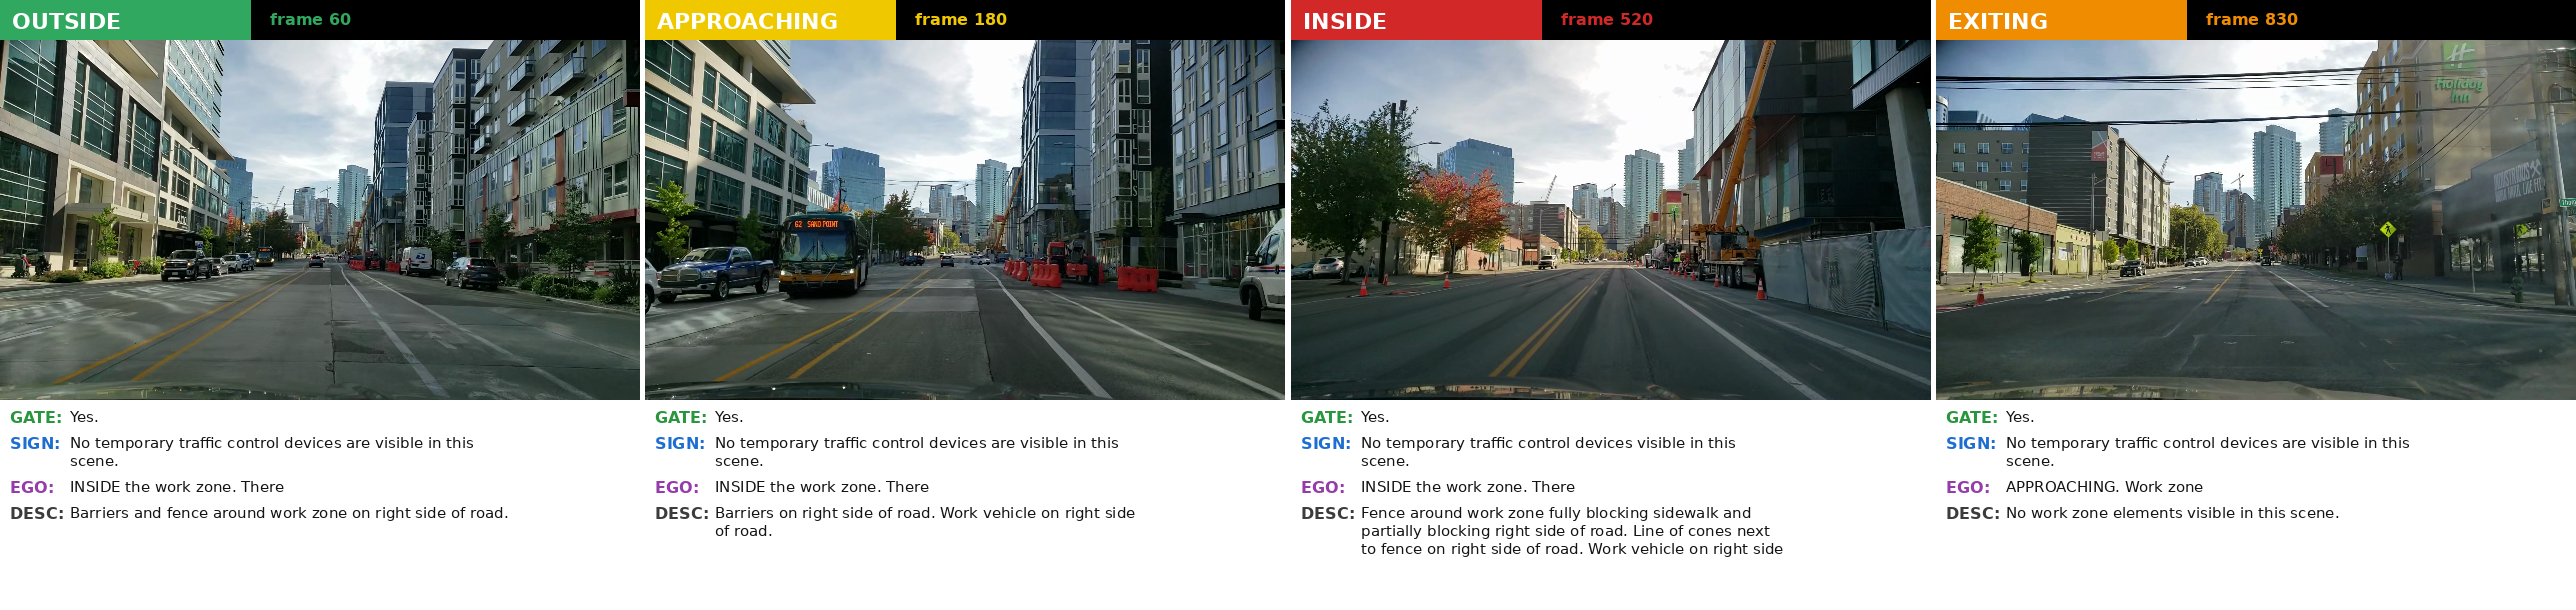
\includegraphics[width=\linewidth]{fig_qualitative.png}
\caption{One continuous validation traversal (Seattle; ground-truth state colored in each banner), with the \emph{actual} per-channel VLM outputs below each frame.  \textsc{outside}: the vehicle has not yet reached the zone, but \textsc{gate} and \textsc{desc} already register the barriers down the block (and \textsc{ego} over-fires ``inside'')---the anticipatory early detection the paper quantifies, and a first illustration of why no single channel is trusted alone.  \textsc{approaching}: barriers and a work vehicle enter the frame; \textsc{gate}+\textsc{desc} corroborate. \textsc{inside}: the vehicle is amid cones and a crane truck, with \textsc{desc} naming the fence and cone line.  \textsc{exiting}: objects recede, \textsc{gate} begins to fade and \textsc{ego} drops back to ``approaching''---the partial-fading trigger---before exit hysteresis returns the state to \textsc{outside}.  \textsc{desc} is truncated to its object--location prefix, the only part the cascade consumes.}
\label{fig:qualitative}
\end{figure}

\section{Cosmos3-Edge deployment and per-model calibration}
\label{supp:calib}

\paragraph{Engines.}  The Cosmos3-Edge reasoner (\path{nemotron_3_dense_vl_text}: 28 layers, hidden 2048, 16 heads, head dim 128, vocab 131{,}072, interleaved-mRoPE disabled with sections $[24,20,20]$) is quantized W4A16 (AWQ INT4, 1.27\,GB); the visual tower stays FP16 (983\,MB) and is frozen at a $26{\times}46$ patch grid, so every frame is resized to $736{\times}416$ (299 vision tokens) rather than the proportional 480\,px resize used for our 2B.  Both are TensorRT engines built with the same embedded runtime~\cite{trtedgellm} on the same device.  Building them required six source patches to the runtime (model-type registration, the multimodal and ViT runners, the visual builder, and the RoPE cache initializer); the patch set is included.  Our 2B pipeline was re-run after patching and reproduces its previous outputs byte-for-byte on an 8-case regression set.

\paragraph{Why per-model calibration is unavoidable.}  \Cref{supp:tab:calib} replays the identical recorded evidence through the identical state machine under both threshold settings.  Only the four integers and the \textsc{ego} switch differ.

\begin{table}[t]
\centering\small
\begin{tabular}{@{}lcc@{}}
\toprule
 & inherited (2B) & recalibrated \\
\midrule
$N$ / $K_\text{enter}$ / $K_\text{exit}$ / $K_\text{fade}$ & 5/3/4/2 & 3/3/2/1 \\
\textsc{ego} channel & on & off \\
\midrule
Frame accuracy & 46.3\% & \textbf{60.5\%} \\
Macro F1 & 0.291 & \textbf{0.484} \\
IoU \textsc{outside} & 0.569 & \textbf{0.675} \\
IoU \textsc{approaching} & 0.241 & \textbf{0.294} \\
IoU \textsc{inside} & 0.021 & \textbf{0.298} \\
IoU \textsc{exiting} & 0.005 & \textbf{0.121} \\
\textsc{inside} recall & 2.1\% & \textbf{34.7\%} \\
\bottomrule
\end{tabular}
\caption{Calibration split (100 videos, 3{,}068 cycles), Cosmos3-Edge, evidence held fixed.  Inheriting our 2B's thresholds understates \textsc{inside} IoU by $14\times$ \emph{on the calibration split itself}, and by $82\times$ on validation (main paper).}
\label{supp:tab:calib}
\end{table}

\paragraph{Evidence dump and offline replay.}  Re-running inference for every configuration would cost GPU-hours.  Instead, at a fixed 1\,s stride, we run all channels on every sampled frame and store parsed evidence (gate, sign keyword, description corroboration, and \textsc{ego}) with ground truth.  Offline replay then sweeps $N\in\{3,5,7,9\}$, $K_\ast\in1..N$, and channel switches in CPU-seconds.  Replay invokes the same state-machine implementation used live through an evidence-level entry point, so the calibrated configuration is exactly the one deployed.

\paragraph{Caveat.}  The dump samples uniformly at 1\,s while the live cascade samples at its own latency-driven cadence, so the window $N$ selected offline corresponds to a slightly different wall-clock span than at run time.  Selection therefore happens under idealized sampling and reporting under real sampling; this is one reason we validate the chosen configuration end-to-end on the held-out split rather than trusting the sweep's own numbers.

\section{Out-of-domain benchmark}
\label{supp:ood}

\paragraph{Footage.}  We recorded 14 California dashcam videos with a different camera and a 1\,Hz GPS sidecar.  Conditions span day, evening, sunset, night, rain, and fog.  A human marked all work-zone sign approaches: 40 timestamps, one excluded as unreadable, leaving \textbf{39}.

\paragraph{Scoring.}  For each annotated timestamp we sample the following 6\,s at 1\,s steps and count a detection if the \textsc{gate} channel answers affirmatively \emph{or} the \textsc{sign} channel transcribes text containing a work-zone keyword, at any sample in the window.  All three systems use the identical window, stride, and decision rule, so the comparison is paired at the level of individual signs.  This measures sign-approach detection, \emph{not} four-state estimation, and is therefore not a substitute for the in-domain benchmark; it isolates whether a system perceives work-zone evidence at all under conditions absent from training.

\paragraph{Trajectory validation.}  GPS sidecars validate the generated ego trajectory (1--4\% displacement error over 6\,s).  We integrate logged speed because position differencing is unstable at this horizon: a 0.1\,s shift changed one estimate from 46.0 to 33.0\,m, while speed integration remained smooth.

\section{Latency, power, and per-city detail}
\label{supp:cost}

\Cref{supp:tab:latency} gives the full per-channel and composite-path latency distributions (60 requests per channel, greedy decoding, 480px input, Jetson AGX Orin MAXN).  Under inference load the module (VDD\_GPU\_SOC + VDD\_CPU\_CV) draws a median 36.5\,W (mean 36.9, p95 41.3, peak 42.5\,W) against a 7.9\,W idle floor, giving per-decision energy of $\sim$3.0\,J (gate), $\sim$8.0\,J (active gate+ego), $\sim$8.7\,J (patrol gate+sign), and $\sim$25.8\,J (full gate+sign+desc corroboration).  Each channel is a separate prefill+decode request that re-encodes the frame; the visual embedding is not shared across a frame's channels, an optimization left for future work.

\begin{table}[t]
\centering\small
\begin{tabular}{@{}lrrrr@{}}
\toprule
Channel (budget) & p50 & p95 & p99 & max \\
\midrule
\textsc{gate} (3)    & 83.4  & 89.9  & 93.7  & 94.0 \\
\textsc{ego} (8)     & 135.5 & 148.8 & 153.1 & 158.5 \\
\textsc{sign} (15)   & 155.1 & 169.4 & 171.1 & 173.5 \\
\textsc{workers} (25)& 313.9 & 341.3 & 344.1 & 344.7 \\
\textsc{desc} (40)   & 468.4 & 508.4 & 514.2 & 515.9 \\
\midrule
patrol (gate+sign)          & 238.5 & 259.3 & --- & --- \\
patrol+corrob.\ (\,+desc)   & 706.8 & 767.7 & --- & --- \\
active (gate+ego)           & 218.8 & 238.8 & --- & --- \\
state-only (gate)           & 83.4  & 89.9  & --- & --- \\
\bottomrule
\end{tabular}
\caption{Per-channel and composite cascade-path latency (ms) on Jetson AGX Orin, greedy decoding, 480px input.}
\label{supp:tab:latency}
\end{table}

\begin{table}[t]
\centering\footnotesize\setlength{\tabcolsep}{2.5pt}
\begin{tabular}{@{}llccccc@{}}
\toprule
System & City & Acc & F1 & appr.\ IoU & ins.\ P & ins.\ R \\
\midrule
VLM (raw)    & Boston  & 61.2\% & 0.444 & 0.124 & 51.6\% & 95.7\% \\
             & Seattle & 66.3\% & 0.520 & 0.224 & 66.2\% & 100\% \\
Det.+CLIP    & Boston  & 63.3\% & 0.469 & 0.113 & 82.0\% & 95.7\% \\
             & Seattle & 61.7\% & 0.462 & 0.152 & 74.2\% & 95.5\% \\
\bottomrule
\end{tabular}
\caption{Per-city breakdown on the validation split (154 Boston, 54 Seattle videos).}
\label{supp:tab:city}
\end{table}

\begin{table}[t]
\centering\small\setlength{\tabcolsep}{3.5pt}
\begin{tabular}{@{}lcccccc@{}}
\toprule
& \multicolumn{3}{c}{Ours (VLM)} & \multicolumn{3}{c}{Det.+CLIP (paired)} \\
\cmidrule(lr){2-4}\cmidrule(lr){5-7}
Tol.\ $\pm k$ & Prec. & Rec. & Acc. & Prec. & Rec. & Acc. \\
\midrule
0  & 0.002 & 0.006 & 0.002 & 0.003 & 0.006 & 0.002 \\
5  & 0.059 & 0.145 & 0.044 & 0.060 & 0.113 & 0.041 \\
15 & 0.122 & 0.298 & 0.094 & 0.157 & 0.296 & 0.114 \\
30 & 0.185 & 0.454 & 0.152 & 0.237 & 0.447 & 0.183 \\
\bottomrule
\end{tabular}
\caption{Transition matching under temporal tolerance ($\pm k$ frames at 30\,fps), both systems under the identical paired latency-honest protocol. Values interleave and stay low for both, confirming that exact transition localization remains open on this benchmark.}
\label{supp:tab:tolerance}
\end{table}

{\small\raggedright
\IfFileExists{ieee_fullname.bst}{\bibliographystyle{ieee_fullname}}{\bibliographystyle{ieeetr}}
\bibliography{references}
}

\end{document}
